\newpage
\begin{center}
  \huge{Codierungstheorie}
\end{center}

\section{Grundbegriffe und einfache Beispiele}
  \subsection{Codierung (Kanalcodierung)}
    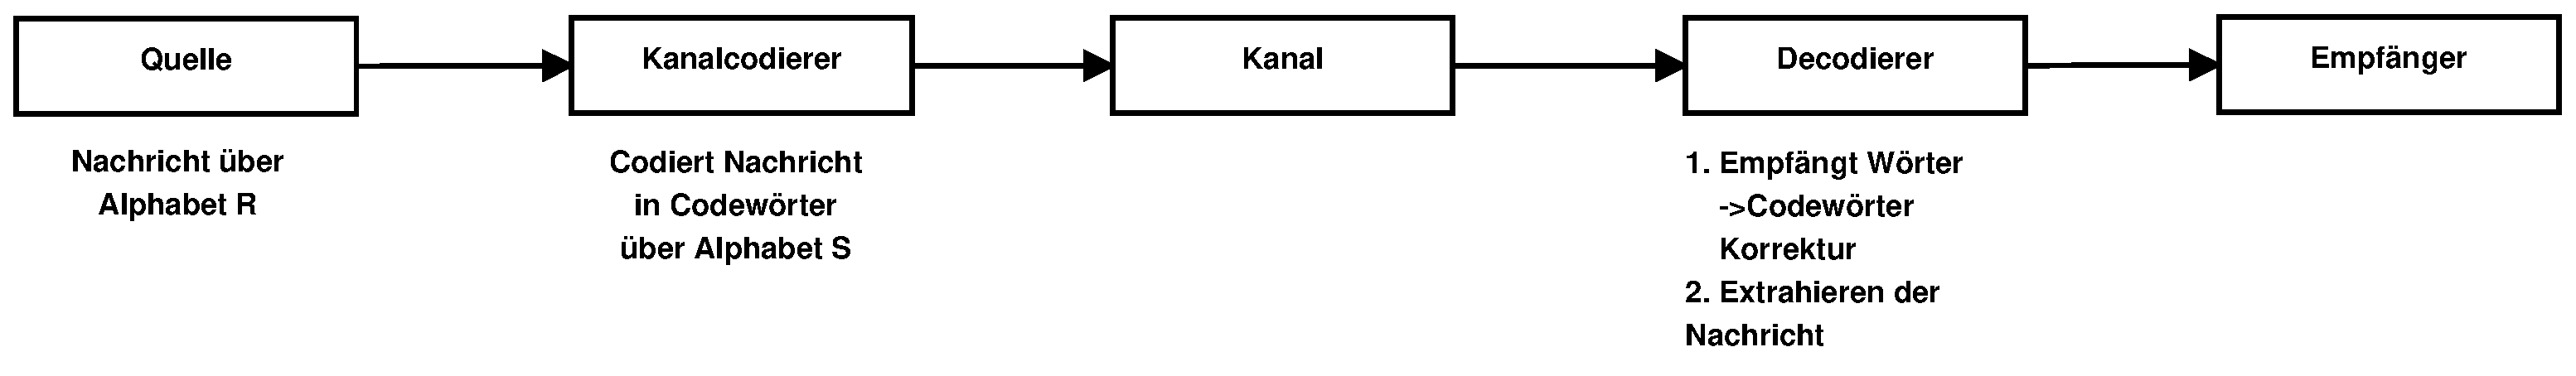
\includegraphics[width=\textwidth]{eps/pic02.eps}
    Ziele:
    \begin{itemize}
      \item Sicherung von Daten bei der Übertragung / Speicherung gegen
      Störungen, Fehler, etc.
      \item Möglichst viele Fehler erkennen und gegebenfalls korrigieren.
      \item Aufwand für Codierung und Decodierung soll nicht zu hoch sein.
    \end{itemize}
    Grundprinzip: Hinzufügen systematischer Redundanz.\\
    Fehlererkennung: Geringe Redundanz
    Fehlerkorrektur: Größere Redundanz, größerer Aufwand
  \subsection{Beispiele}
    \begin{enumerate}[a)]
      \item Parity- Check- Code
        $R=\lrc{0,1}$\\
        Nachricht wird in Blöcke von Länge $k$ zerlegt. Füge an jeden Block Bit
        an, so dass die Anzahl der Einsen im Block der Länge $k+1$ gerade ist
        (also 1 für ungerade, 0 für gerade).\\
        $k=2$:\\
        $00\rightarrow000\\
        01\rightarrow011\\
        10\rightarrow101\\
        11\rightarrow110\\$
        1 Fehler wird erkannt (kann nicht korrigiert werden). 2 Fehler können
        nicht erkannt werden.
      \item Wiederholungscode: Nachricht zerlegt in Blöcke der Länge $k$. Jeder
        Block wird $m$ mal gesendet. $k=2$, $m=3$\\
        $01\rightarrow000000\\
        01\rightarrow010101\\
        10\rightarrow101010\\
        11\rightarrow111111\\$
        1 Fehler lässt sich korrigieren.
      \item Codiere Blöcke der Länge 2 wiefolgt:\\
        $00\rightarrow00000\\
        01\rightarrow01101\\
        10\rightarrow10110\\
        11\rightarrow11011\\$
        1- Fehler- korrigierend:\\
        Decodierung: Such das \gqm{nächste} Codeword zum empfangenen Wort. Je
        zwei Codewörter unterscheiden sich an mindestens 3 Stellen.\\
        2- Fehler- erkennend: Kann jedoch nicht korrigiert werden, da Abstand
        zu zwei gültigen Worten 2 ist.
    \end{enumerate}
  \subsection{GTIN- Prüfzifferncode (GTIN-13)}
    \begin{enumerate}[a)]
      \item GTIN=Global Trade Item Number (früher EAN-13)\\
        12- stelliger Code, $R=S=\lrc{0,...,9}$. Erste 12 Ziffern ensprechen
        Information, 13. Ziffer ist die Prüfziffer\\
        $c_1...c_{13}:c_1...c_{12}$\\
        Herstellungsland (in der Regel die ersten drei Ziffern, Deutschland:
        400-440)\\
        Hersteller (in der Regel $c_4,...,c_8$ (4-6 Ziffern)\\
        Produkt (in der Regel $c_9,...,c_{12}$ (3-5 Ziffern)\\
        $c_{13}$ wird so gewählt, dass gilt:
        $c_1+3c_2+c_3+3c_4+...+c_{11}+3c_{12}+c_{13}\equiv 0(\mod 10)$\\
        $c_{13}=(-c_1+3c_2-c_3-...-3c_12)\mod 10$\\
        Änderung einer Ziffer wird erkannt. $x\mapsto 3x\mod 10$ ist bijektiv
        ($\ggT(3,10)=1$)
    \end{enumerate}
